%\documentclass[landscape,a0b,final,a4resizeable]{a0poster}
\documentclass[landscape,a0b,final]{a0poster}
%\documentclass[portrait,a0b,final,a4resizeable]{a0poster}
%\documentclass[portrait,a0b,final]{a0poster}
%%% Option "a4resizeable" makes it possible to resize the
%   poster by the command: psresize -pa4 poster.ps poster-a4.ps
%   For final printing, please remove option "a4resizeable" !!

\usepackage{epsfig}
\usepackage{multicol}
\usepackage{pstricks,pst-grad}
\usepackage{graphicx,psfrag}
\usepackage{graphics}
\usepackage{amsmath}
\usepackage{amsthm}
\usepackage{amsfonts}

\newtheorem{example}{Example}
\newtheorem{assumption}{Assumption}
\newtheorem{definition}{Definition}
\newtheorem{theorem}{Theorem}
\newtheorem{lemma}{Lemma}


%%%%%%%%%%%%%%%%%%%%%%%%%%%5

\usepackage{eso-pic}
\usepackage{graphicx}
\usepackage{color}
\usepackage{type1cm}


%%%%%%%%%%%%%%%%%%%%%%%%%%%%%%%%%%%%%%%%%%%%%%%%%%%%
%%%               WaterMark                       %%%
%%%%%%%%%%%%%%%%%%%%%%%%%%%%%%%%%%%%%%%%%%%%%%%%%%%%
%\makeatletter
%  \AddToShipoutPicture{%
%    \setlength{\@tempdimb}{.5\paperwidth}%
%    \setlength{\@tempdimc}{.5\paperheight}%
%    \setlength{\unitlength}{1pt}%
%    \put(\strip@pt\@tempdimb,\strip@pt\@tempdimc){%
%      \makebox(0,0){\rotatebox{45}{\textcolor[gray]{0.15}{\includegraphics[width=120cm,angle=0]{SU_Seal_Card_pos.eps}}}}
%    }
%}
%\makeatother



%%%%%%%%%%%%%%%%%%%%%%%%%%%%%%%%%%%%%%%%%%%
% Definition of some variables and colors
%\renewcommand{\rho}{\varrho}
%\renewcommand{\phi}{\varphi}
\setlength{\columnsep}{3cm}
\setlength{\columnseprule}{2mm}
\setlength{\parindent}{0.0cm}



%%%%%%%%%%%%%%%%%%%%%%%%%%%%%%%%%%%%%%%%%%%%%%%%%%%%
%%%               Background                     %%%
%%%%%%%%%%%%%%%%%%%%%%%%%%%%%%%%%%%%%%%%%%%%%%%%%%%%

\newcommand{\background}[3]{
  \newrgbcolor{cgradbegin}{#1}
  \newrgbcolor{cgradend}{#2}
  \psframe[fillstyle=gradient,gradend=cgradend,
  gradbegin=cgradbegin,gradmidpoint=#3](0.,0.)(1.\textwidth,-1.\textheight)
}



%%%%%%%%%%%%%%%%%%%%%%%%%%%%%%%%%%%%%%%%%%%%%%%%%%%%
%%%                Poster                        %%%
%%%%%%%%%%%%%%%%%%%%%%%%%%%%%%%%%%%%%%%%%%%%%%%%%%%%

\newenvironment{poster}{
  \begin{center}
  \begin{minipage}[c]{0.98\textwidth}
}{
  \end{minipage} 
  \end{center}
}



%%%%%%%%%%%%%%%%%%%%%%%%%%%%%%%%%%%%%%%%%%%%%%%%%%%%
%%%                pcolumn                       %%%
%%%%%%%%%%%%%%%%%%%%%%%%%%%%%%%%%%%%%%%%%%%%%%%%%%%%

\newenvironment{pcolumn}[1]{
  \begin{minipage}{#1\textwidth}
  \begin{center}
}{
  \end{center}
  \end{minipage}
}



%%%%%%%%%%%%%%%%%%%%%%%%%%%%%%%%%%%%%%%%%%%%%%%%%%%%
%%%                pbox                          %%%
%%%%%%%%%%%%%%%%%%%%%%%%%%%%%%%%%%%%%%%%%%%%%%%%%%%%

%\newrgbcolor{lcolor}{0. 0. 0.80}
\newrgbcolor{lcolor}{1 1 1}
\newrgbcolor{gcolor1}{1. 1. 1.}
\newrgbcolor{gcolor2}{.80 .80 1.}

\newcommand{\pbox}[4]{
\psshadowbox[#3]{
\begin{minipage}[t][#2][t]{#1}
#4
\end{minipage}
}}



%%%%%%%%%%%%%%%%%%%%%%%%%%%%%%%%%%%%%%%%%%%%%%%%%%%%
%%%                myfig                         %%%
%%%%%%%%%%%%%%%%%%%%%%%%%%%%%%%%%%%%%%%%%%%%%%%%%%%%
% \myfig - replacement for \figure
% necessary, since in multicol-environment 
% \figure won't work

\newcommand{\myfig}[3][0]{
\begin{center}
  \vspace{1.5cm}
  \includegraphics[width=#3\hsize,angle=#1]{#2}
  \nobreak\medskip
\end{center}}

\newcommand{\myfigp}[3][0]{
\begin{center}
  \vspace{1.5cm}
  \includegraphics[width=#3\hsize]{#1}
  \includegraphics[width=#3\hsize]{#2}
  \nobreak\medskip
\end{center}}



%%%%%%%%%%%%%%%%%%%%%%%%%%%%%%%%%%%%%%%%%%%%%%%%%%%%
%%%                mycaption                     %%%
%%%%%%%%%%%%%%%%%%%%%%%%%%%%%%%%%%%%%%%%%%%%%%%%%%%%
% \mycaption - replacement for \caption
% necessary, since in multicol-environment \figure and
% therefore \caption won't work

%\newcounter{figure}
\setcounter{figure}{1}
\newcommand{\mycaption}[1]{
  \vspace{0.5cm}
  \begin{quote}
    {{\sc Figure} \arabic{figure}: #1}
  \end{quote}
  \vspace{1cm}
  \stepcounter{figure}
}



%%%%%%%%%%%%%%%%%%%%%%%%%%%%%%%%%%%%%%%%%%%%%%%%%%%%%%%%%%%%%%%%%%%%%%
%%% Begin of Document
%%%%%%%%%%%%%%%%%%%%%%%%%%%%%%%%%%%%%%%%%%%%%%%%%%%%%%%%%%%%%%%%%%%%%%

\begin{document}





\newrgbcolor{lightblue}{0. 0. 0.80}
\newrgbcolor{white}{1. 1. 1.}
\newrgbcolor{whiteblue}{1 1 1}
\newrgbcolor{red}{0.6431 0 0.1137}
\newrgbcolor{whitered}{0.6431 0 0.1137}




\begin{poster}

\background{0.6431 0 0.1137}{1. 1. 1.}{0.5}
\vspace*{2.5cm}
%%%%%%%%%%%%%%%%%%%%%
%%% Header
%%%%%%%%%%%%%%%%%%%%%
\begin{center}
\begin{pcolumn}{0.992}

\pbox{0.95\textwidth}{}{linewidth=4mm,framearc=0.3,linecolor=red,fillstyle=gradient,gradangle=0,gradbegin=white,gradend=white,gradmidpoint=1.0,framesep=1em}{

%%% DARPA-DSO logo
\begin{minipage}[c][4.5cm][c]{0.13\textwidth}
  \begin{center}
    
\includegraphics[width=13cm,angle=0]{Darpadsologo}
  \end{center}
\end{minipage}
%%% AA logo
\begin{minipage}[c][4.5cm][c]{0.14\textwidth}
  \begin{center}
    %\includegraphics[width=8cm,angle=0]{SU_Seal_Card_pos}
    \vspace{5mm}
    
\includegraphics[width=12cm,angle=0]{aalogo}
  \end{center}
\end{minipage}
%%% Title
\begin{minipage}[c][9cm][c]{0.46\textwidth}
  \begin{center}
    {\sc \Huge Cutoff Phenomena in Chaotic Dynamics}\\[10mm]
    {\Large Tzu-Chen Liang\\[7.5mm]
     Department of Aeronautics and Astronautics, Stanford University }
  \end{center}
\end{minipage}
%%% Stanford logo
\begin{minipage}[c][4.5cm][c]{0.10\textwidth}
  \begin{center}
    \hspace{2cm}
    \includegraphics[width=8cm,angle=0]{SU_Seal_Card_pos}
  \end{center}
\end{minipage}
%%% DynaRUM logo
\begin{minipage}[c][9cm][c]{0.17\textwidth}
  \begin{center}
    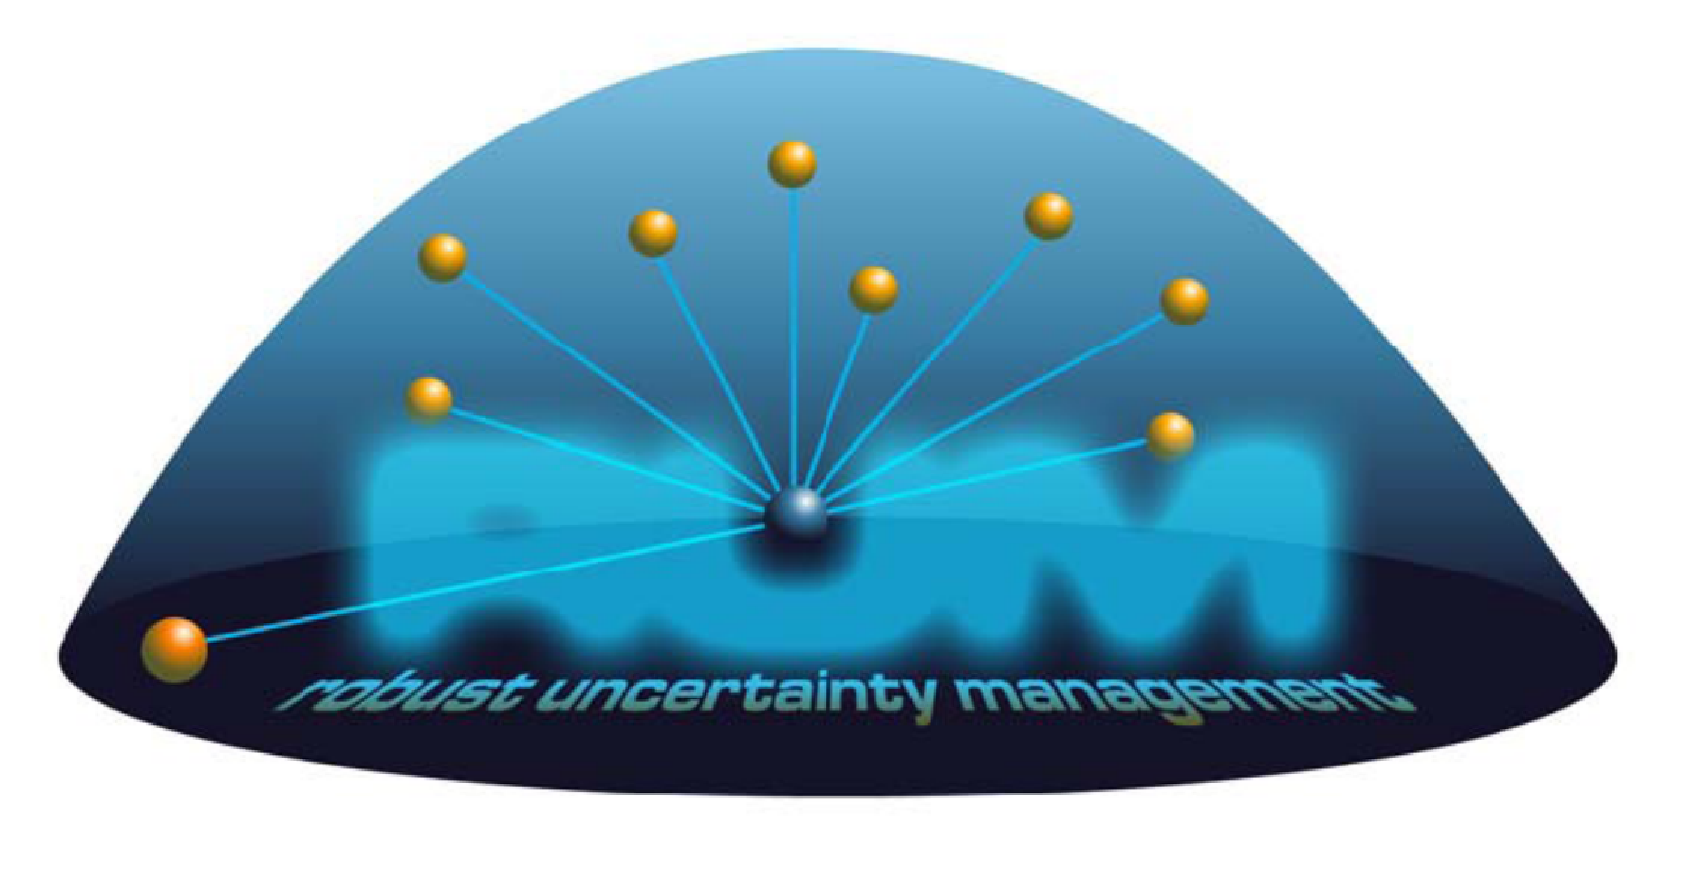
\includegraphics[width=15cm,angle=0]{Dynarumlogo}
  \end{center}
\end{minipage}
} 



%\pbox{0.95\textwidth}{}{linewidth=4mm,framearc=0.3,linecolor=red,fillstyle=gradient,gradangle=0,gradbegin=white,gradend=white,gradmidpoint=1.0,framesep=1em}{








\end{pcolumn}
\end{center}


\vspace*{2cm}



%%%%%%%%%%%%%%%%%%%%%
%%% Content
%%%%%%%%%%%%%%%%%%%%%
%%%%%%%%%%%%%%%%%%%%%%%%%%%%%%%%
%Here is the 1st column
%%%%%%%%%%%%%%%%%%%%%%%%%%%%%%%%

\begin{center}
\begin{pcolumn}{0.32}
\pbox{0.9\textwidth}{65cm}{linewidth=4mm,framearc=0.1,linecolor=red,fillstyle=gradient,gradangle=0,gradbegin=white,gradend=white,gradmidpoint=1.0,framesep=1em}{

%%% Introduction
\begin{center}\pbox{0.8\textwidth}{}{linewidth=2mm,framearc=0.1,linecolor=red,fillstyle=gradient,gradangle=0,gradbegin=white,gradend=whitered,gradmidpoint=1.0,framesep=1em}{\begin{center}\bfseries{\large{Introduction}}\end{center}}\end{center}
\vspace{1.25cm}
%%%%%%%%%%%%%%%%%%%%%%%%%%%%%%%%%%%%%%%%%%%%%%%%%%%%%%%%%%%%%%%%%%%%%%%%%%%%%%%%%%%%%%%%%%%%%%%%
%Introduction begins here


%Introduction ends here
%%%%%%%%%%%%%%%%%%%%%%%%%%%%%%%%%%%%%%%%%%%%%%%%%%%%%%%%%%%%%%%%%%%%%%%%%%%%%%%%%%%%%%%%%%%%%%%%%




%%% Cutoff 
\vspace{0.7cm}\begin{center}\pbox{0.8\textwidth}{}{linewidth=2mm,framearc=0.1,linecolor=red,fillstyle=gradient,gradangle=0,gradbegin=white,gradend=whitered,gradmidpoint=1.0,framesep=1em}{\begin{center}\bfseries{\large{Cutoff Phenomenon}}\end{center}}\end{center}\vspace{1cm}
%%%%%%%%%%%%%%%%%%%%%%%%%%%%%%%%%%%%%%%%%%%%%%%%%%%%%%%%%%%%%%%%%%%%%%%%%%%%%%%%%%%%%%%%%%%%%%%%
%section begins here


%section ends here
%%%%%%%%%%%%%%%%%%%%%%%%%%%%%%%%%%%%%%%%%%%%%%%%%%%%%%%%%%%%%%%%%%%%%%%%%%%%%%%%%%%%%%%%%%%%%%%%%





}
\end{pcolumn}
\begin{pcolumn}{0.32}
%%%%%%%%%%%%%%%%%%%%%%%%%%%%%%%%
%Here is the 2nd column
%%%%%%%%%%%%%%%%%%%%%%%%%%%%%%%%
\pbox{0.9\textwidth}{65cm}{linewidth=4mm,framearc=0.1,linecolor=red,fillstyle=gradient,gradangle=0,gradbegin=white,gradend=white,gradmidpoint=1.0,framesep=1em}{



\begin{center}\pbox{0.8\textwidth}{}{linewidth=2mm,framearc=0.1,linecolor=red,fillstyle=gradient,gradangle=0,gradbegin=white,gradend=whitered,gradmidpoint=1.0,framesep=1em}{\begin{center}\bfseries{\large{Tent Map and Logistic Map Cutoffs}}\end{center}}\end{center}\vspace{1cm}

%%%%%%%%%%%%%%%%%%%%%%%%%%%%%%%%%%%%%%%%%%%%%%%%%%%%%%%%%%%%%%%%%%%%%%%%%%%%%%%%%%%%%%%%%%%%%%%%
%Section begins here










%Section ends here
%%%%%%%%%%%%%%%%%%%%%%%%%%%%%%%%%%%%%%%%%%%%%%%%%%%%%%%%%%%%%%%%%%%%%%%%%%%%%%%%%%%%%%%%%%%%%%%%
}
\end{pcolumn}
\begin{pcolumn}{0.32}
%%%%%%%%%%%%%%%%%%%%%%%%%%%%%%%%
%Here is the 3rd column
%%%%%%%%%%%%%%%%%%%%%%%%%%%%%%%%
\pbox{0.9\textwidth}{65cm}{linewidth=4mm,framearc=0.1,linecolor=red,fillstyle=gradient,gradangle=0,gradbegin=white,gradend=white,gradmidpoint=1.0,framesep=1em}{

\begin{center}\pbox{0.8\textwidth}{}{linewidth=2mm,framearc=0.1,linecolor=red,fillstyle=gradient,gradangle=0,gradbegin=white,gradend=whitered,gradmidpoint=1.0,framesep=1em}{\begin{center}\bfseries{\large{Cutoff in Advection-Diffusion Simulation}}\end{center}}\end{center}\vspace{1.25cm}

%%%%%%%%%%%%%%%%%%%%%%%%%%%%%%%%%%%%%%%%%%%%%%%%%%%%%%%%%%%%%%%%%%%%%%%%%%%%%%%%%%%%%%%%%%%%%%%%
%Section begins here











%Section ends here
%%%%%%%%%%%%%%%%%%%%%%%%%%%%%%%%%%%%%%%%%%%%%%%%%%%%%%%%%%%%%%%%%%%%%%%%%%%%%%%%%%%%%%%%%%%%%%%%

% Future Work
\begin{center}\pbox{0.8\textwidth}{}{linewidth=2mm,framearc=0.1,linecolor=red,fillstyle=gradient,gradangle=0,gradbegin=white,gradend=whitered,gradmidpoint=1.0,framesep=1em}{\begin{center}\bfseries{\large{Future Work}}\end{center}}\end{center}\vspace{0.5cm}



\vspace{-0.5cm}
% References
%\bibliographystyle{plain}
%\bibliography{mixingbib}
%\nocite{Thiffeault2004}
%\nocite{Mezic2005}

}
\end{pcolumn}
\end{center}



\vspace*{2cm}



\end{poster}

\end{document}

